
\section{Introduction}
The \ac{TCA} implementation for the \ac{CMR} is one that heavily utilizes geometry and a rigid-body model assumption, while also placing an emphasis on relying on minimal assumptions/data about the environment and avoiding computationally complex calculations on input data from sensors, cameras, etc. There were various reasons as to why some of these assumptions/choices were made and why the agreed upon implementation was deemed the best choice for the given scenario. \cite{tractl} Figure~\ref{traction_control:algorithms:scarecrow} shows a testbed version of the \ac{CMR}.

\begin{figure}[htbp]
	\centering
	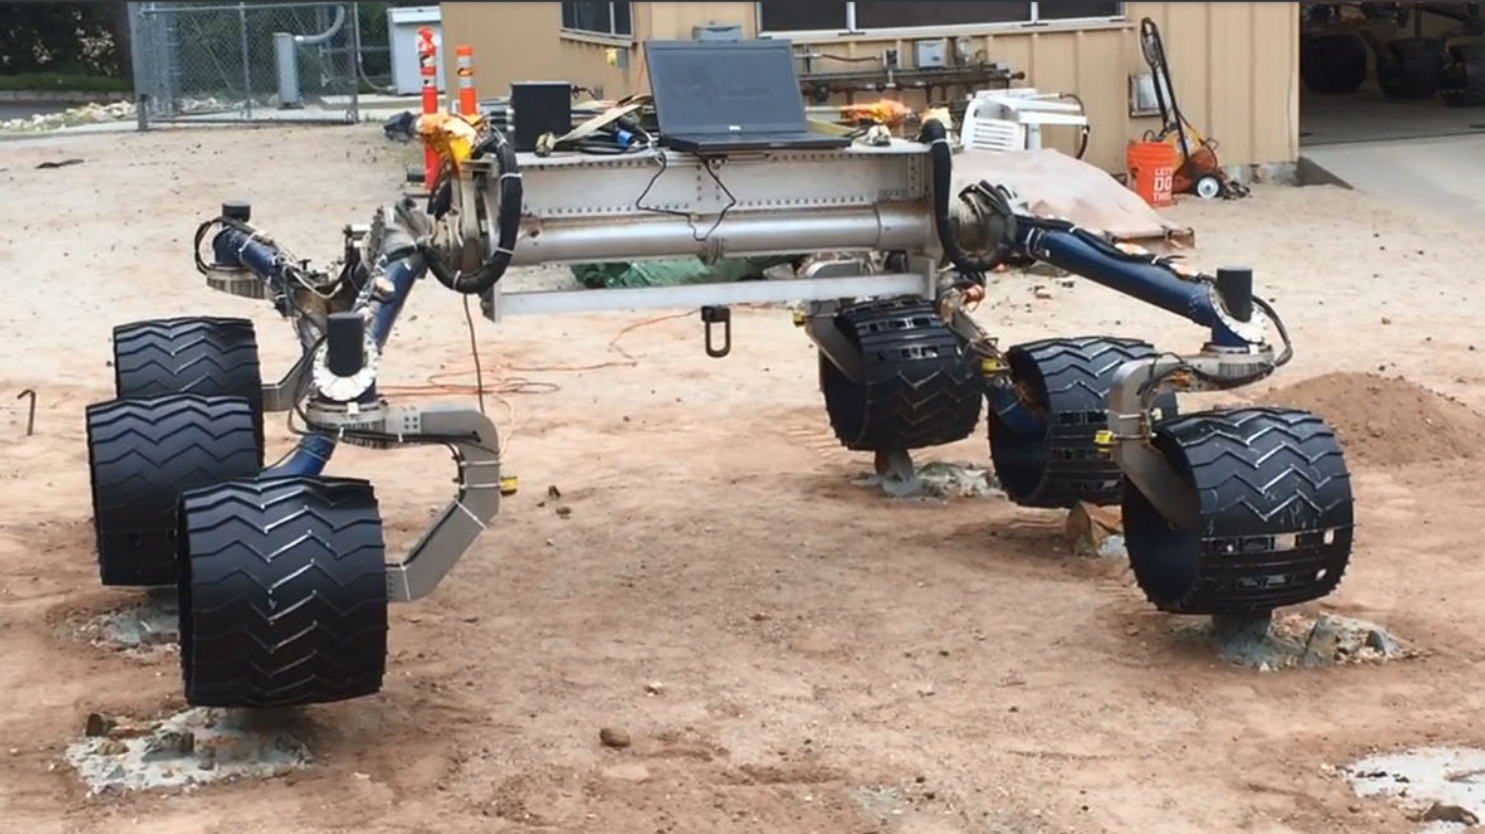
\includegraphics[width=.9\textwidth]{sections/algorithms/images/scarecrow_testbed.png}
	\caption{The Scarecrow Testbed Rover, a Rover Kinematically Similar to the \acl{CMR} \cite{tractl}}
	\label{traction_control:algorithms:scarecrow}
\end{figure}

\section{Design Limitations and Considerations}
It is important to note that the need for this \ac{TCA} was not discovered until after the flight system was actively engaging in its mission on the Martian surface, while ground control was observing telemetry of its use. Therefore, it was impossible to make any physical modifications to the \ac{CMR}, only software could be remotely flashed to it. \\

However, there are still ramifications to having this additional routine run on the \ac{CMR}. The limited computational resources available to do so must be considered carefully, so as to not interfere with existing processes being ran, and the implementation chosen has to have enough resources to perform the task it needs to as well. The team responsible for solving the problem at hand clarified some of these issues and how it restricted their choices for strategies to solve the problem. For example, the rover ``does not include force or torque sensors on the mobility subsystem, nor can it measure slip with high enough frequency to be able to react to it.'' \cite{tractl} \\

Some of the characteristics and assumptions of the \ac{CMR} and its \ac{TCA} implementation are discussed in the following sections.

\section{Ackermann Steering Model}
Modeling vehicles using the Ackermann steering model is a common practice, including for the \ac{CMR}. Even thought it adds slightly more complex geometric modeling, the mechanical steering system can be implemented relatively easily, and there are benefits to doing so. \\

Figure~\ref{traction_control:algorithms:ackermann-steering} illustrates a basic vehicle that is modeled using Ackermann steering, where the left image has the wheels positioned such that the vehicle will move straight, while the right image would cause the vehicle to turn counter-clockwise. Important to note is that when in a turning position, the front wheels are not turned to the same angle as one another, because of the nonzero distance between them. They are positioned such that the direction that both wheels are pointing are normal to a common center point called the \ac{ICC}, so that when the vehicle turns, the left and right wheels follow two different circular arcs, but both of their centers are at the \ac{ICC}.

\begin{figure}[H]
	\centering
	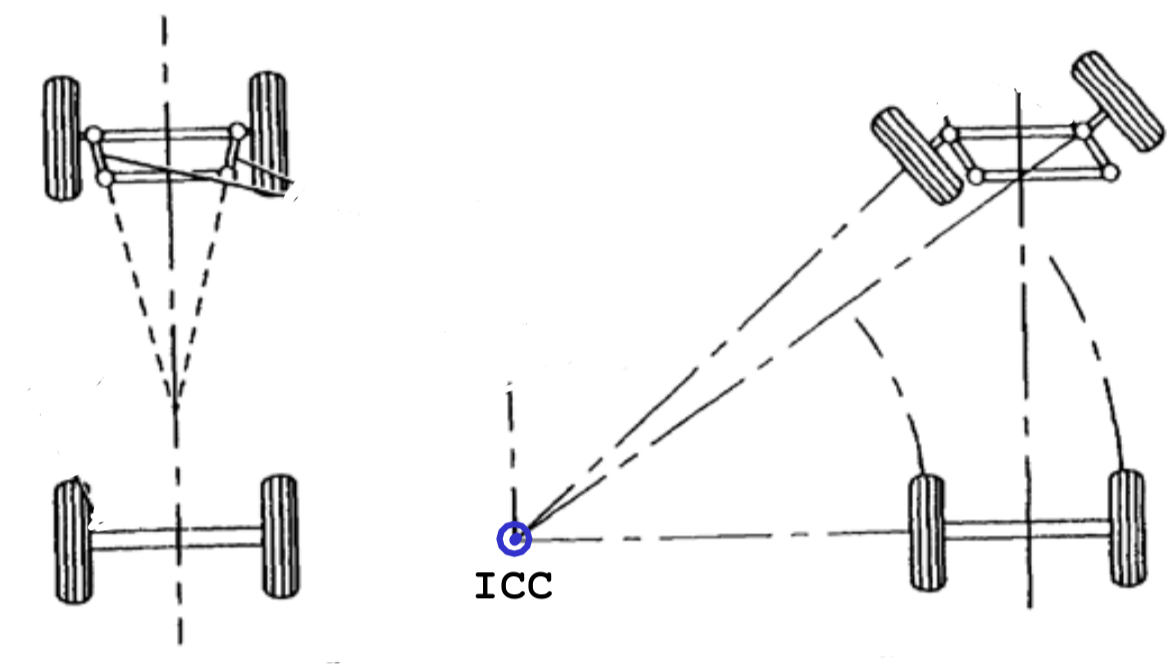
\includegraphics[width=.9\textwidth]{sections/algorithms/images/ackermann_steering.png}
	\caption{A Vehicle with Ackermann Steering Going Straight (Left) and in a Turning Position(Right)}
	\label{traction_control:algorithms:ackermann-steering}
\end{figure}

The benefit to this is that, assuming all the wheels' velocities are coordinated and in an ideal world, at no point while traveling in these flat, circular arcs will a wheel slip. Less slippage means less unpredictable behavior, such as a wheel slipping over a rough surface. However, the assumption that the \ac{CMR} would only be traversing terrain that could be modeled as flat is what led to the need for the \ac{TCA}, as excessive slippage occurred due to the reality that the terrain was non-negligible. As one wheel would traverse over a rock and then back down, it traveled a longer distance. \\

The Ackermann steering model by itself does not account for this extra distance and this caused the wheel slippage, which damaged them at an alarming rate. This is how the \ac{TCA} can be used to improve the model, so that when rough terrain is being traversed, the wheel(s) doing so can be sped up accordingly.

\section{Rigid-Body Model Assumption}
The rigid-body model assumption says that a body of some sturdy material can be assumed to maintain it shape, and that a force/torque that it can expect to encounter will not deform it to a degree that needs to be accounted for. This is not true in reality, but in scenarios like these, the deformation can be negligible. \\

Making this assumption can be extremely beneficial when implementing an algorithm like \ac{TCA} because it heavily simplifies the math needed to represent vectors in different coordinate frames.

\section{Coordinate Frame Notation}
%
%TO-DO, add: \\
% 1.) description of what a coordinate frame is and why they're used \\
% 2.) \ac{CMR} frame notation \\
% 3.) mention differences in \ac{SRR} frames \\
% 4.) maybe more \\

Coordinate frames are useful in robotics for the purpose of keeping track of the robot positions, orientations, and velocities in space. These frames can be translated from  a reference to another frame, such as from the base robot frame to each individual leg frame. Robotics often uses Cartesian coordinates, so the coordinate frames are created with an origin, x, y, and z axes. \\

To be able to show the relative position and orientation of one frame to another, geometric relationships between them need to be found. A rotation matrix can be used to show the relative orientation between two frames. For example, the orientation of the 1st frame $o_{1}x_{1}y_{1}z_{1}$ with respect to the base frame $o_{0}x_{0}y_{0}z_{0}$ can be written with the rotation matrix:
\begin{equation}\label{traction_control:algorithms:r01}
	R^{0}_{1} = [x^{0}_{1} | y^{0}_{1} | z^{0}_{1}]
\end{equation}

One way to compute the rotation matrix is with the entries being in terms of angle $\theta$. The second way is to project the 1st frame on the 0 frame which uses the dot product.  The dot products with respect of the 1st frame onto the 0 frame can be shown as
\begin{equation}
	x^{0}_{1} = \left[\begin{array}{c}
				x_{1}\cdot x_{0} \\
			    x_{1}\cdot y_{0} \\
			    x_{1}\cdot z_{0}
				\end{array} \right],
			%
	y^{0}_{1} = \left[\begin{array}{c}
				y_{1}\cdot x_{0} \\
				y_{1}\cdot y_{0} \\
				y_{1}\cdot z_{0}
	\end{array} \right],
			%
	z^{0}_{1} = \left[\begin{array}{c}
				z_{1}\cdot x_{0} \\
				z_{1}\cdot y_{0} \\
				z_{1}\cdot z_{0}
	\end{array} \right]
\end{equation}

There are three basic rotation matrices- about the x-axis, y-axis, and z-axis. With respect to angle $\theta$, these rotation matrices are defined in
Equations~\ref{traction_control:algorithms:rx}, \ref{traction_control:algorithms:ry}, \ref{traction_control:algorithms:rz}. 
These 3 rotations are also called the roll$(\phi)$, pitch $(\theta)$, and yaw$(\psi)$ matrices. The order of rotation is through yaw (x,$(\psi)$),pitch (y,$(\theta)$), and roll (z,$(\phi)$. \\

\begin{equation}
	R_{x,\theta} = \left[\begin{array}{ccc}
				1 & 0 & 0 \\
				0 & cos(\theta) & -sin(\theta)  \\
				0 & sin(\theta) & cos(\theta) 
				\end{array}\right]
	\label{traction_control:algorithms:rx}
\end{equation}

\begin{equation}
	R_{y,\theta} = \left[\begin{array}{ccc}
		cos(\theta) & 0 & sin(\theta) \\
		0 & 1 & 0 \\
		-sin(\theta) & 0 & cos(\theta) 
	\end{array}\right]
	\label{traction_control:algorithms:ry}
\end{equation}

\begin{equation}
	R_{z,\theta} = \left[\begin{array}{ccc}
		cos(\theta) & sin(\theta) & 0 \\
		sin(\theta) & cos(\theta) & 0 \\
		0 & 0 & 1 \\
	 
	\end{array}\right]
	\label{traction_control:algorithms:rz}
\end{equation}\\

After finding both the position and orientation of a frame, they can be put into a homogeneous transformation matrix. This can comprise of a series of rigid motions, which are pure translations and pure rotations only. The transformation matrix consists of the rotation between the frames (top 3x3), the distance (right 3x1 column vector), and the bottom row being matrix identity to allow a series of multiplications. Figure~\ref{traction_control:algorithms:basicT} shows the homogeneous transformation matrix. 

\begin{equation}
	H^{0}_{n} = \left[\begin{array}{cc}
			R^{0}_{n} & d^{0}_{n}\\
			0 & 1 
			\end{array}\right]
		\label{traction_control:algorithms:basicT}
\end{equation}


The rover, like any robot, has coordinate frames to define its position and rotation matrices.
 Figure~\ref{traction_control:algorithms:coordinates-side} shows these frames from the left side of the robot. A top view is also provided as Figure~\ref{traction_control:algorithms:coordinates-top}.

\begin{figure}[H]
	\centering
	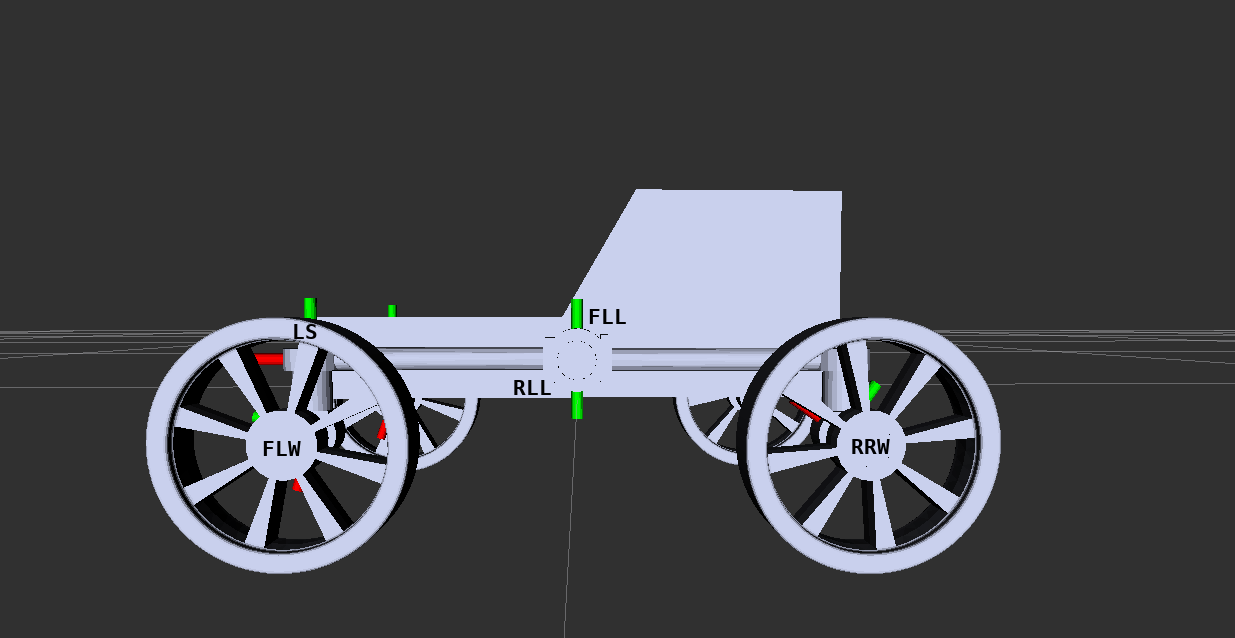
\includegraphics[scale=0.35, width=.7\textwidth]{sections/algorithms/images/srr_side.png}
	\caption{Side View of the Robot Model and its Coordinate Frames}
	\label{traction_control:algorithms:coordinates-side}
\end{figure}
 
\begin{figure}[H]
	\centering
	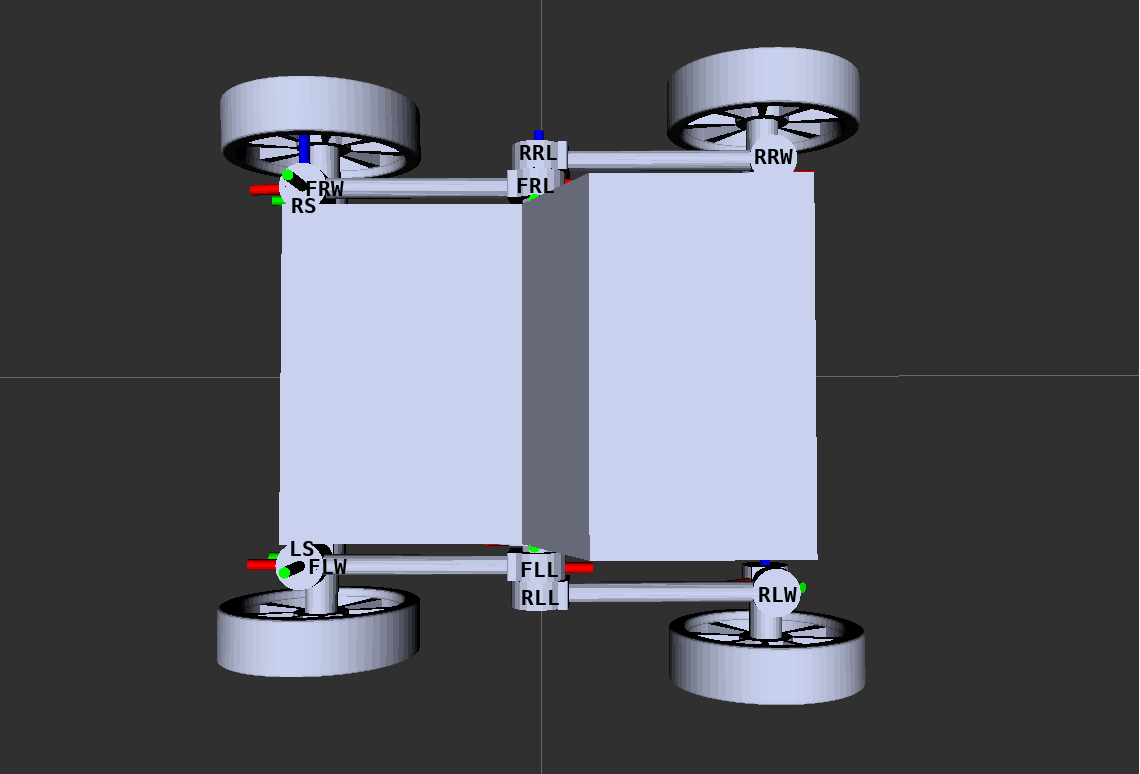
\includegraphics[scale=0.3]{sections/algorithms/images/srr_top.png}
	\caption{Side View of the Robot Model and its Coordinate Frames}
	\label{traction_control:algorithms:coordinates-top}
\end{figure}
 
A summary of the acronyms for the coordinate frames used in Figures~\ref{traction_control:algorithms:coordinates-side} and~\ref{traction_control:algorithms:coordinates-top} are seen below in Table~\ref{table:1}.
\begin{table}[H]
\begin{center}
	\begin{tabular}{|c|c|} 
		\hline    
		Label & Name \\
		\hline
		FLL & Front Left Leg \\
		FRL & Front Right Leg \\
		RLL & Rear Left Leg \\
		RRL & Rear Right Leg \\
		FLW & Front Left Wheel \\
		FRW & Front Right Wheel \\
		RLW & Rear Left Wheel \\
		RRW & Rear Right Wheel \\
		LS  & Left Steering \\ 
		RS  & Right Steering \\ 
	    \hline
	\end{tabular}
 	\caption{\label{table:1} Table of Acronyms for Model Axes}  	
\end{center}
\end{table}

The rover model can be drawn to show its geometry in a simple manner. Depicted from its side, there is the pivot joint from the chassis in the center. Two legs are connected to the the center pivot joint. The front leg also has a revolute joint at its end to be able to steer the front wheels.

The difference between this model and the Curiosity Rover is that the Curiosity Rover has a third leg, which can be defined as the rocker joint and bogie joints. The legs are designed much differently as compared to the early model of the Sample-Return Rover. The SRR only has the center pivot joint.

As seen in Figure~\ref{traction_control:algorithms:side-diagram},the diagram is of the left side of the rover, and the front is facing left. Wheel centers are denoted with $A_{i}$. The lengths of each leg are shown with $l_{i}$. Angles of specific areas are denoted by either $\psi$, k, or $\delta$. 


\begin{figure}[H]
	\centering
	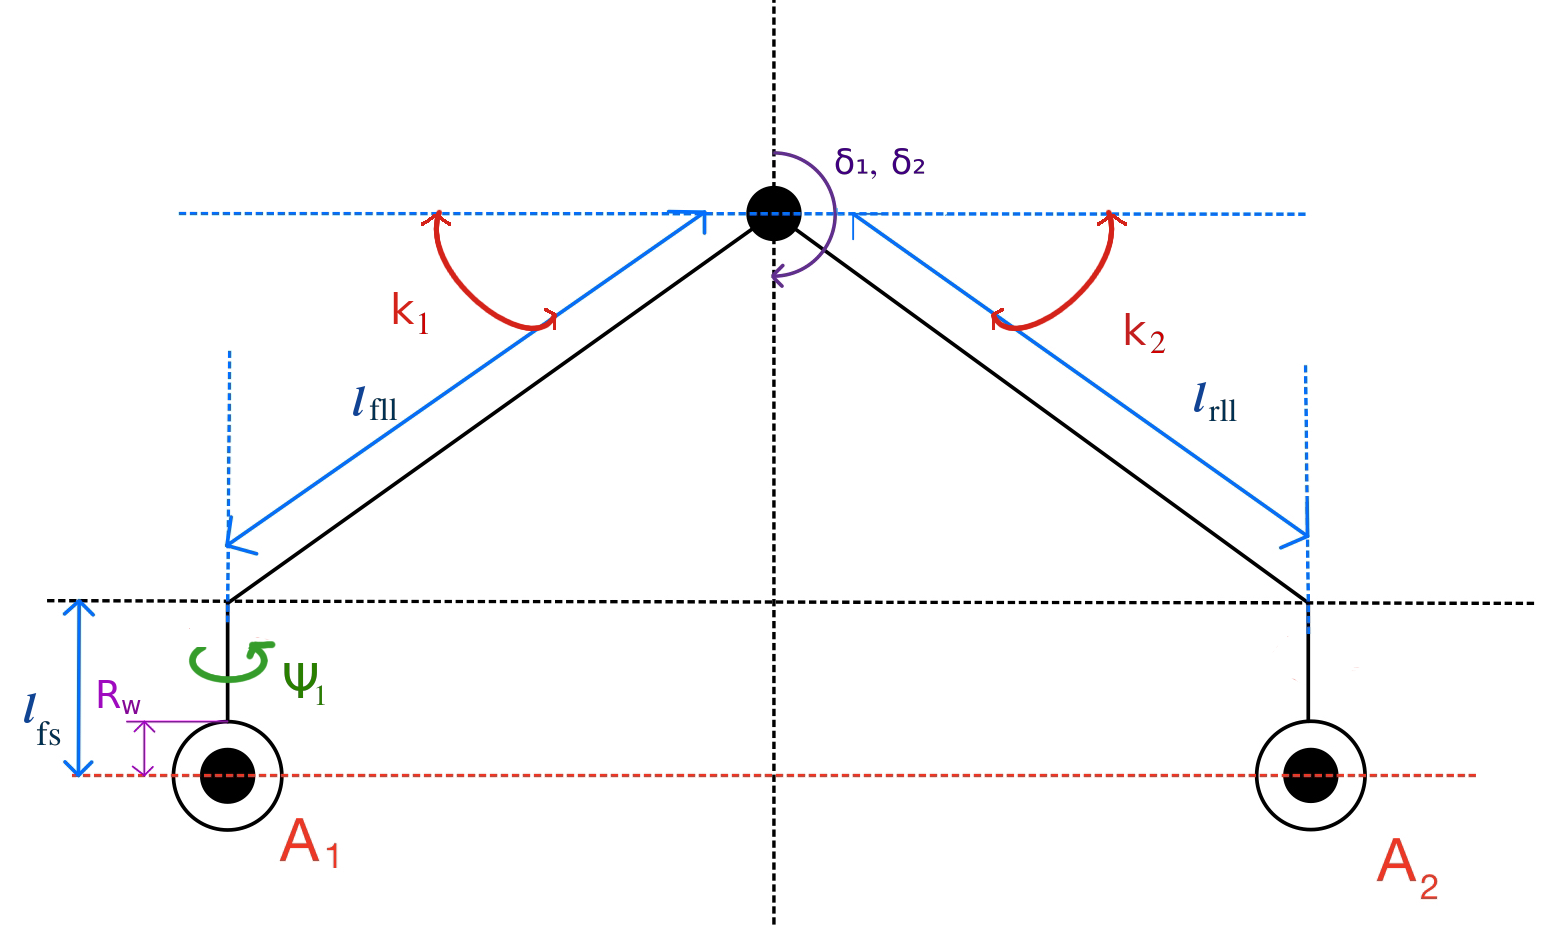
\includegraphics[scale=0.3]{sections/algorithms/images/side-diagram.png}	
	\caption{Side Diagram of the Rover Model on Flat Ground}	
	\label{traction_control:algorithms:side-diagram}
\end{figure}

\begin{table}[H]
\begin{center}\label{table:2}
	\begin{tabular}{| >{\centering\arraybackslash} m{1.2in} | >{\centering\arraybackslash} m{4.5in} |} 
		\hline
		Symbol & Description \\
		\hline
		A1 & Wheel 1 - Front Left \\
		A2 & Wheel 2 - Rear Left \\
		$R_{w}$ & Wheel Radius \\
		$\psi_{1}$ & Front Steering Angle \\
		$k_{1}$ & Angle between Front Leg and Chassis x-axis on Flat Ground \\
		$k_{2}$ & Angle between Rear Leg and Chassis x-axis on Flat Ground \\
		$l_{fs}$ & Front Steering Leg Length \\ 
		$l_{fll}$ & Front Left Leg Length \\ 
		$l_{rll}$ & Rear Left Leg Length \\ 
		$\delta_{1}$ & Front Left Leg Pivot Angle    \\
		$\delta_{2}$ & Rear Left Leg Pivot Angle   \\
		\hline
	
	\end{tabular}
\caption{Description of Symbol Nomenclature}
\end{center}
\end{table}


\section{Calculations}
